\documentclass[12pt, a4paper]{report}
\usepackage[utf8]{inputenc}
\usepackage[english, russian]{babel}

\usepackage{graphicx}
\usepackage{listings}
\usepackage{color}

\usepackage{amsmath}
\usepackage{pgfplots}
\usepackage{url}
\usepackage{flowchart}
\usepackage{tikz}
\DeclareGraphicsExtensions{.pdf,.png,.jpg,.svg}
\usetikzlibrary{shapes, arrows}

\usepackage{pgfplotstable}

\renewcommand\contentsname{Содержание}

\usepackage{geometry}
\geometry{left=3cm}
\geometry{right=1cm}
\geometry{top=2cm}
\geometry{bottom=2cm}

\lstset{ %
language=Python,                 % выбор языка для подсветки (здесь это С)
basicstyle=\small\sffamily, % размер и начертание шрифта для подсветки кода
numbers=left,               % где поставить нумерацию строк (слева\справа)
numberstyle=\tiny,           % размер шрифта для номеров строк
stepnumber=1,                   % размер шага между двумя номерами строк
numbersep=-5pt,                % как далеко отстоят номера строк от         подсвечиваемого кода
backgroundcolor=\color{white}, % цвет фона подсветки - используем         \usepackage{color}
showspaces=false,            % показывать или нет пробелы специальными     отступами
showstringspaces=false,      % показывать или нет пробелы в строках
showtabs=false,             % показывать или нет табуляцию в строках
frame=single,              % рисовать рамку вокруг кода
tabsize=2,                 % размер табуляции по умолчанию равен 2 пробелам
captionpos=t,              % позиция заголовка вверху [t] или внизу [b] 
breaklines=true,           % автоматически переносить строки (да\нет)
breakatwhitespace=false, % переносить строки только если есть пробел
escapeinside={\%*}{*)},   % если нужно добавить комментарии в коде
keywordstyle=\color{blue}\ttfamily,
stringstyle=\color{red}\ttfamily,
commentstyle=\color{green}\ttfamily,
morecomment=[l][\color{magenta}]{\#},
columns=fullflexible }

\usepackage{titlesec}
\titleformat{\chapter}[hang]{\LARGE\bfseries}{\thechapter{.} }{0pt}{\LARGE\bfseries}
\titleformat*{\section}{\Large\bfseries}
\titleformat*{\subsection}{\large\bfseries}

\begin{document}

    \begin{titlepage}

        \begin{center}
            \Large
            {\sl Государственное образовательное учреждение высшего профессионального образования\\
            	{\bf«Московский государственный технический университет имени Н.Э. Баумана»\\
            		(МГТУ им. Н.Э. Баумана)}}
            \noindent\rule{\textwidth}{2pt}


            \vspace{3cm}

			{\scshape\LARGE Лабораторная работа №1 \par}
			\vspace{0.3cm}	
			{\scshape\LARGE «Анализ алгоритмов» \par}
			\vspace{1.5cm}
			{\huge\bfseries Расстояние Левенштейна и Дамерау-Левенштейна \par}
			\vspace{2cm}
			\begin{flushleft}
			\Large Студент: Нгуен Фыок Санг\\
			\Large Группа ИУ7-56Б\\
			Преподаватель:  Волокова Л. Л.\\
			Оценка:
			\end{flushleft} 
			
			
		
			\vfill
			\Large \textit {Москва, 2020 г.}
            
        \end{center}

    \end{titlepage}
	
	\tableofcontents
	
	\chapter*{Введение}
	\addcontentsline{toc}{chapter}{Введение}
	
	В современном мире почти каждый человек пользуются компьютером и Интернетом в частности. Люди пишут текст в документах, выполняют поиск в поисковых системах, ищут переводы слов и текстов в онлайн-словарях. В таких ситуациях человек часто делает орфографические ошибки или опечатки, и на их исправление он тратит своё время. Чтобы этого избежать, в подобных системах есть опции поиска ошибок и автоисправления. Для такой опции необходим поиск расстояния между строками по алгоритмам Левенштейна и Дамерау-Левенштейна. Также эта задача необходима и в программировании (например, для сравнения текстовых файлов или файлов кода в системах контроля версий) и в биоинформатике (например, для сравнения белков, генов и хромосом).

    \chapter{Аналитическая часть}

	\section{Задачи}
	{\bfЦель лабораторной работы:} Разработать и сравнить алгоритмы поиска расстоянии Левенштейна и Дамерау-Левенштейна. \\
	\\
	Задачи работы
	\begin{enumerate}
		\item Дать математическое описание расстояний
		\item Описать алгоритмы
		\item Реализовать алгоритмы 
		\item Провести тестирование
		\item Осуществить замеры процессорного времени работы алгоритмов
	\end{enumerate}

	\section{Описание алгоритмов}
	\subsection{Расстояние Левенштейна}
	Расстояние Левенштейна определяет минимальное количество операций, необходимых для превращения одной строки в другую, среди которых:
	\begin{itemize}
		\item вставка (I - insert);
		\item удаление (D - delete);
		\item замена (R - replace).
	\end{itemize}
	
	\begin{equation}
	\label{formula_leven}
	D(S_{1}[i], S_{2}[j]) =
		\begin{cases}
		i, \ if\ j = 0\\
		j, \ if\ i = 0\\
		min \begin{cases}
		D(S_{1}[i-1], S_{2}[j] + 1)\\
		D(S_{1}[i], S_{2}[j-1]+1)\\
		D(S_{1}[i-1], S_{2}[j-1])+
			\begin{cases}
				1, if\  S_{1}[i] \neq S_{2}[j]\\
				0, else
			\end{cases}
		\end{cases}  i > 0,\  j > 0
	\end{cases}
	\end{equation}

	\subsection{Расстояние Дамерау-Левенштейна}
	Расстояние Дамерау-Левенштейна является модификацией расстояние Левенштейна. К исходному набору возможных операций добавляется операция транспозиции (T - transpose), или перестановка двух соседних символов.
	
	При вычислении расстояния Дамерау-Левенштейна в рекурретную формулу вносится дополнительное соотношение в минимум:
	\begin{equation}
	\label{damerau_eq}
	D(S_{1}[i-2], S_{2}[j-2])+1
	\end{equation}
	Соотношение ~(\ref{damerau_eq}) вносится в выражение только при выполнении следующих условий:
	\begin{equation}
	\label{damerau_conditions}
	\begin{cases}
		i > 1,\ j > 1\\
		S_{1}[i] = S_{2}[j-1]\\
		S_{1}[i-1] = S_{2}[j]
	\end{cases}	
	\end{equation}
	
	Таким образом получаем следующую рекурретную формулу:
	
	\begin{equation}
	\label{formula_damerau}
	D(S_{1}[i],S_{2}[j]) = \begin{cases}
	i\ if\ j = 0\\
	j\ if\ i = 0\\
	min \begin{cases}
		D(S_{1}[i-1], S_{2}[j] + 1)\\
		D(S_{1}[i], S_{2}[j-1]+1)\\
		D(S_{1}[i-1], S_{2}[j-1])+
			\begin{cases}
				1, if\  S_{1}[i] \neq S_{2}[j]\\
				0, else
			\end{cases}\\
		D(S_{1}[i-2], S_{2}[j-2])+1
	\end{cases} & \mbox{if ~(\ref{damerau_conditions})}\\	
	min \begin{cases}
		D(S_{1}[i-1], S_{2}[j] + 1)\\
		D(S_{1}[i], S_{2}[j-1]+1)\\
		D(S_{1}[i-1], S_{2}[j-1]+
			\begin{cases}
				1, if\  S_{1}[i] \neq S_{2}[j]\\
				0, else
			\end{cases}
	\end{cases} & \mbox{else}\\
	\end{cases}
	\end{equation}

	\chapter{Конструкторская часть}
	
	\section{Схемы алгоритмов}
	На рисунках 2.1 - 2.5 представлены схемы алгоритмов реализаций алгоритмов поиск расстояния между строками.
	\begin{figure}[ht!]
		\centering
		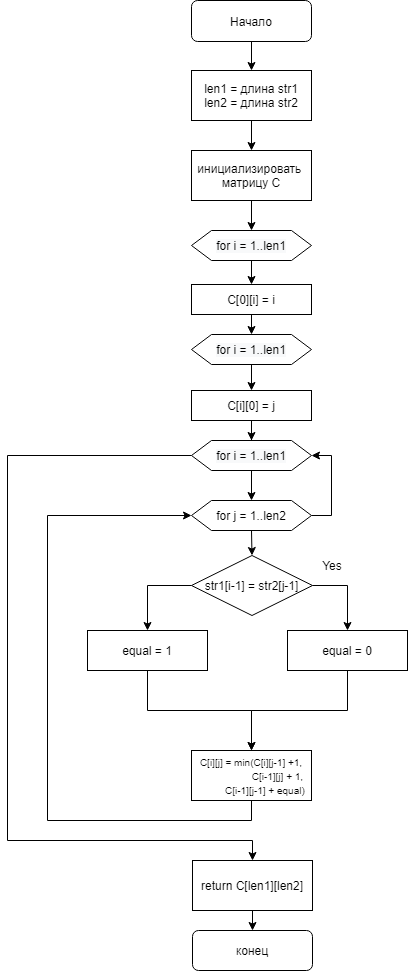
\includegraphics[scale=0.5]{Dia1.png}
		\caption{Матричная реализация алгоритма Левенштейна}
		\label{fig:leven}
	\end{figure}

	\begin{figure}[ht!]
		\centering
		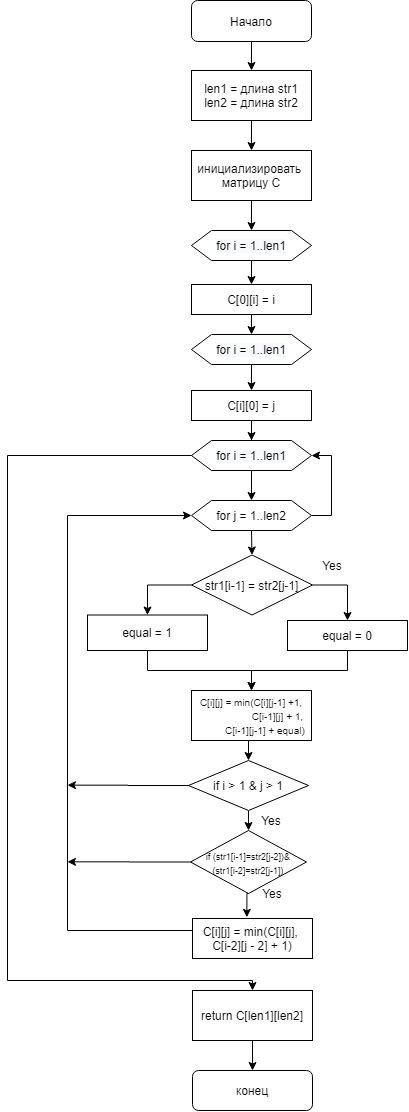
\includegraphics[scale=0.6]{Dia2.png}
		\caption{Матричная реализация алгоритма Дамерау-Левенштейна}
		\label{fig:damleven}
	\end{figure}

	\begin{figure}
		\centering
		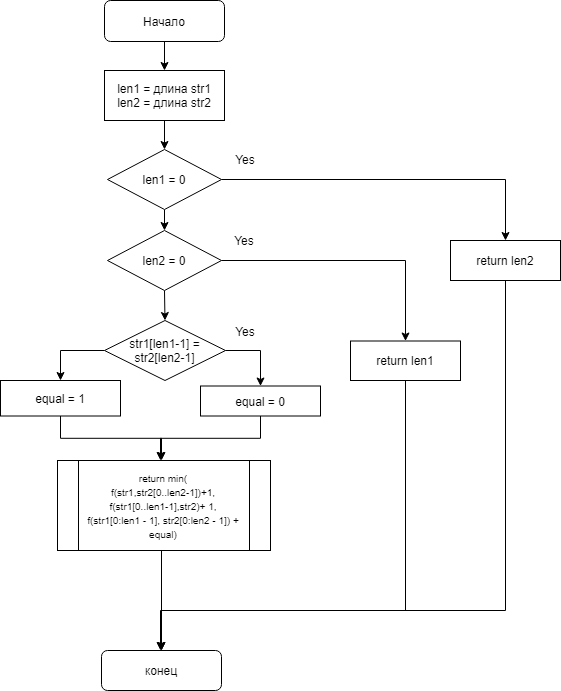
\includegraphics[scale=0.7]{Dia3.png}
		\caption{Рекурсивная реализация алгоритма Левенштейна}
		\label{fig:reclevenr}
	\end{figure}

	\begin{figure}
		\centering
		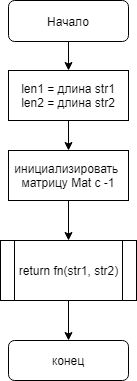
\includegraphics[scale=0.7]{Dia5.png}
		\caption{Рекурсивная реализация алгоритма Левенштейна с заполнением матрицу}
		\label{fig:reclevenrtab1}
	\end{figure}

	\begin{figure}
		\centering
		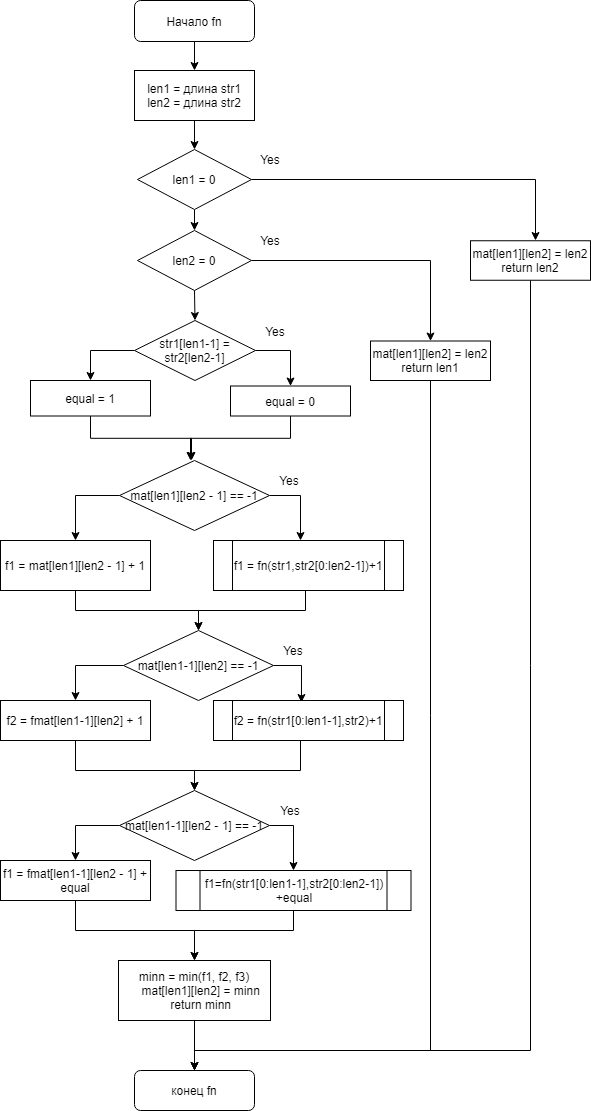
\includegraphics[scale=0.6]{Dia4.png}
		\caption{Рекурсивная реализация алгоритма Левенштейна с заполнением матрицу}
		\label{fig:reclevenrtab2}
	\end{figure}

	\newpage
	
	\chapter{Технологическая часть}
	\section{Средства реализации}
	Для реализации программы был использован язык Python. Для замера процессорного времени была использована функция time() из библиотеки time.
	\section{Реализации алгоритмов}
	На листингах 3.1 - 3.4 представлены коды реализации алгоритмов поиска расстояния.
	\begin{lstlisting}[label=some-code,caption=Матричная реализация алгоритма Левенштейна]
		
	def levenshtein(str1, str2):
	
		len1 = len(str1)
		len2 = len(str2)
	
		C = [[0 for i in range(len2 + 1)] for j in range(len1 + 1)]
	
		for i in range(0, len2 + 1):
			C[0][i] = i
	
		for i in range(0, len1 + 1):
			C[i][0] = i
	
		for i in range(1, len1 + 1):
			for j in range(1, len2 + 1):
				if (str1[i - 1] == str2[j - 1]):
					equal = 0
				else:
					equal = 1
	
				C[i][j] = min(C[i][j-1] + 1,
							  C[i-1][j] + 1,
							  C[i-1][j-1] + equal)
		#matrix_print(str1, str2, C)
		return C[len1][len2]
	\end{lstlisting}

	\begin{lstlisting}[label=some-code,caption=Матричная реализация алгоритма Дамерау-Левенштейна]
	
	def damerau_levenshtein(str1, str2):
		len1 = len(str1)
		len2 = len(str2)
		
		C = [[0 for i in range(len2 + 1)] for j in range(len1 + 1)]
		
		for i in range(0, len2 + 1):
			C[0][i] = i
		
		for i in range(0, len1 + 1):
			C[i][0] = i
		
		for i in range(1, len1 + 1):
			for j in range(1, len2 + 1):
				if (str1[i - 1] == str2[j - 1]):
					equal = 0
				else:
					equal = 1
		
				C[i][j] = min(C[i][j-1] + 1,
							  C[i-1][j] + 1,
							  C[i-1][j-1] + equal)
		
				if (i > 1 and j > 1 and str1[i - 1] == str2[j - 2] and str1[i - 2] == str2[j - 1]):
					C[i][j] = min(C[i][j], C[i-2][j - 2] + 1)
		
		#matrix_print(str1, str2, C)
		return C[len1][len2]
	
	\end{lstlisting}

	\begin{lstlisting}[label=some-code,caption=Рекурсивная реализация алгоритма Левенштейна]
	
	def levenshtein_recursive(str1, str2):
		len1 = len(str1)
		len2 = len(str2)
		
		if (len1 == 0):
			return len2
		if (len2 == 0):
			return len1
		
		is_equal = 1
		if (str1[len1 - 1] == str2[len2 - 1]):
			is_equal = 0
		
		return min(levenshtein_recursive(str1, str2[0 : len2 - 1]) + 1,
						levenshtein_recursive(str1[0 : len1 - 1], str2) + 1,
						levenshtein_recursive(str1[0:len1 - 1], str2[0:len2 - 1]) + is_equal)
	
	\end{lstlisting}

	\begin{lstlisting}[label=some-code,caption=Рекурсивная реализация с заполнением матрицу алгоритма Левенштейна]
		def levenshtein_recursive_table(str1, str2):
			res = levenshtein_recursive_tab(str1, str2)
			delattr(levenshtein_recursive_tab, "mat")
		return res
		
		def levenshtein_recursive_tab(str1, str2):
			fn = levenshtein_recursive_tab
			len1 = len(str1)
			len2 = len(str2)
			if not hasattr(fn, "mat"):
				fn.mat = [[-1 for i in range(len2 + 1)] for i in range(len1 + 1)]
		
			if (len1 == 0):
				fn.mat[len1][len2] = len2
				return len2
			
			if (len2 == 0):
				fn.mat[len1][len2] = len1
				return len1
		
			f1, f2, f3 = 0, 0, 0
			is_equal = 1
		
			if (str1[len1 - 1] == str2[len2 - 1]):
				is_equal = 0
		
			if (fn.mat[len1][len2 - 1] == -1):
				f1 = fn(str1, str2[0 : len2 - 1]) + 1
			else:
				f1 = fn.mat[len1][len2 - 1] + 1
		
			if (fn.mat[len1 - 1][len2] == -1):
				f2 = fn(str1[0 : len1 - 1], str2) + 1
			else:
				f2 = fn.mat[len1 - 1][len2] + 1
		
			if (fn.mat[len1 - 1][len2 - 1] == -1):
				f3 = fn(str1[0:len1 - 1], str2[0:len2 - 1]) + is_equal
			else:
				f3 = fn.mat[len1 - 1][len2 - 1] + is_equal
		
			minn = min(f1, f2, f3)
			fn.mat[len1][len2] = minn
			return minn
		
	\end{lstlisting}


	\newpage

	\section{Тесты}
	Для проверки корректности работы были подготовлены функциональные тесты, представленные в таблице 3.1. В данной таблице $\lambda$ означает пустую строку, а числа в столбцах "Ожидание" и "Результат" соответствуют результатам работы алгоритмов в следующем порядке:
	\begin{enumerate}
		\item Расстояние Левенштейна.
		\item Расстояние Дамерау-Левенштейна.
	\end{enumerate}

	\begin{table}[ht!]
		\caption{Функциональные тесты}
		\begin{center}
			\begin{tabular}{|c|c|c|c|}
			\hline
			\bf{Строка 1} & \bf{Строка 2} & \bf{Ожидание} & \bf{Результат}\\\hline
			$\lambda$ & $\lambda$ & 0 0 & 0 0\\\hline
			$\lambda$ & а & 1 1 & 1 1\\\hline
			а & $\lambda$ & 1 1 & 1 1\\\hline
			а & а & 0 0 & 0 0\\\hline
			а & b & 1 1 & 1 1\\\hline
			аbc & acb & 2 1 & 2 1\\\hline
			1234 & 567 & 4 4 & 4 4\\\hline
			human & cat & 4 4 & 4 4\\\hline
			\end{tabular}
		\end{center}
	\end{table}

	В результате проверки все реализации алгоритмов прошли все поставленные функциональные тесты.

	\chapter{Исследованая часть}
	\section{Сравнение работы алгоритмов}
	
	\begin{table}[ht!]
		\caption{Время работы матричных реализаций алгоритмов (ms) процессора}
		\begin{center}
			\pgfplotstabletypeset[
			col sep=semicolon,
			string type,
			columns/Size/.style={column name=Длина слова, column type={|c}},
			columns/Leven/.style={column name=Алг. Лев-на, column type={|c}},
			columns/Damerau/.style={column name=Алг. Дамерау Лев-на, column type={|c}},
			columns/Damerautable/.style={column name=Алг. Лев-на (Рекурсивнoй с мат), column type={|c|}},
			every head row/.style={before row=\hline,after row=\hline},
			every last row/.style={after row=\hline},
			]{Text.txt}
		\end{center}
	\end{table}
	
	\begin{figure}[ht!]
		\begin{tikzpicture}
		\begin{axis}
			[%title = График времени работы матричных реализаций алгоритмов Левенштейна и Дамерау-Левенштейна,
			table/col sep = semicolon,
			xlabel={Количество символов},
			ylabel={Время (ms)},
			ymin = 0,
			legend pos=outer north east,
			ymajorgrids=true,
			grid style=dashed]
			\addplot[color=red, mark=*] table[x={Size}, y={Leven}] {Text.txt};
			\addplot[color=blue, mark=*] table[x={Size}, y={Damerau}] {Text.txt};
			\addplot[color=green, mark=*] table[x={Size}, y={Damerautable}] {Text.txt};
			\legend{Алгоритм Левенштейна, Алгоритм Дамерау-Левенштейна, Рек. aлгоритм Левенштейна с матрицей}
		\end{axis}
		\end{tikzpicture}
		\caption{График времени работы матричных реализаций алгоритмов Левенштейна и Дамерау-Левенштейна}
	\end{figure}
	
	Алгоритм Левенштейна выигрывает по времени. Алгоритм Дамерау-Левенштейна выполняется дольше за счёт добавления небольшого количества операций.
	Рекурсивный алгоритм Левенштейна с заполнением матрицу самый долгии.
   
	\section{Сравнение работы реализаций алгоритма Левенштейна}
	
	
	\begin{table}[ht!]
		\begin{center}
			\caption{Время (ms) работы реализаций алгоритма Левенштейна  процессора}
			\pgfplotstabletypeset[
			col sep=semicolon,
			string type,
			columns/Size/.style={column name=Длина слова, column type={|c}},
			columns/Matrix/.style={column name=Матричная реализация, column type={|c}},
			columns/Recursive/.style={column name=Рекурсивная реализация, column type={|c|}},
			every head row/.style={before row=\hline,after row=\hline},
			every last row/.style={after row=\hline},
			]{DamerauTime.csv}
		\end{center}
	\end{table}

	\begin{figure}[ht!]
		\begin{tikzpicture}
			\begin{axis}
			[%title = График времени работы матричной реализации алгоритма Левенштейна,
			table/col sep = semicolon,
			xlabel={Количество символов},
			ymin = 0,
			legend pos=outer north east,
			ymajorgrids=true,
			grid style=dashed]
			\addplot[color=red, mark=*] table[x={Size}, y={Matrix}] {Time.csv};
			\end{axis}
		\end{tikzpicture}
		\caption{График времени работы матричной реализации алгоритма Левенштейна}
	\end{figure}
	
	\begin{figure}[ht!]
		\begin{tikzpicture}
			\begin{axis}
			[%title = График времени работы рекурсивной реализации алгоритма Левенштейна,
			table/col sep = semicolon,
			xlabel={Количество символов},
			ylabel={Время(ms)},
			ymin = 0,
			legend pos=outer north east,
			ymajorgrids=true,
			grid style=dashed]
			\addplot[color=blue, mark=*] table[x={Size}, y={Recursive}] {Time.csv};
			\end{axis}
		\end{tikzpicture}
		\caption{График времени работы рекурсивной реализации алгоритма Левенштейна}
	\end{figure}

	
 	Время выполнения рекурсивной реализации алгоритма резко возрастает с увеличением длины слов. Можно сделать вывод о том, что матричная реализация алгоритма значительно эффективнее рекурсивной при любой длине слова.

	\section{Вывод}
	
	\chapter*{Заключение}

	\begin{enumerate}
		\item Дано математическое описание расстояний
		\item Описаны алгоритмы
		\item Реализованы алгоритмы 
		\item Провести тестирование
		\item Осущественны замеры процессорного времени работы алгоритмов
	\end{enumerate}
	

\end{document}
